\documentclass{juliacon}

\setcounter{page}{1}

\usepackage{mathrsfs}
\usepackage{amssymb,amstext,amsfonts,amsmath}

\usepackage{todonotes}
\newcommand{\todoi}[2][]{\todo[inline,#1]{#2}}
\newcommand{\todoq}[2][]{\todo[inline,color=blue!20!white,#1]{#2}}

\usepackage{xspace}
\usepackage[labelformat=simple]{subfig}
\renewcommand{\thesubfigure}{(\alph{subfigure})}

\usepackage{calc}
\usepackage{graphicx,import}

\usepackage{comment}

% no number in references section
\usepackage[square,sort,comma,numbers]{natbib}

% algorithms-pseudocode
\usepackage{jlcode}
\usepackage{listings}

\lstset{
	language=Julia,
	basicstyle=\ttfamily\footnotesize,
	numberstyle=\scriptsize,
	backgroundcolor=\color{gray!10},
	frame=single,
	tabsize=2,
	rulecolor=\color{black!30},
	title=\lstname,
	escapeinside={\%(*}{*)},
	breaklines=true,
	breakatwhitespace=true,
	framextopmargin=2pt,
	framexbottommargin=2pt,
	extendedchars=true,
	inputencoding=utf8,
	columns=fullflexible,
}

% letters
\newcommand{\bfa}{{\bf a}}
\newcommand{\bfA}{{\bf A}}
%
\newcommand{\bfb}{{\bf b}}
\newcommand{\bfB}{{\bf B}}
%
\newcommand{\bfc}{{\bf c}}
\newcommand{\bfC}{{\bf C}}
%
\newcommand{\bfd}{{\bf d}}
\newcommand{\bfD}{{\bf D}}
%
\newcommand{\bfe}{{\bf e}}
\newcommand{\bfE}{{\bf E}}
%
\newcommand{\bff}{{\bf f}}
\newcommand{\bfF}{{\bf F}}
%g
\newcommand{\bfg}{{\bf g}}
\newcommand{\bfG}{{\bf G}}

\newcommand{\bfi}{{\bf i}}
\newcommand{\bfI}{{\bf I}}
%
\newcommand{\bfh}{{\bf h}}
\newcommand{\bfH}{{\bf H}}
%
\newcommand{\bfk}{{\bf k}}
\newcommand{\bfK}{{\bf K}}
%
\newcommand{\bfl}{{\bf l}}
\newcommand{\bfL}{{\bf L}}
% m
\newcommand{\bfm}{{\bf m}}
\newcommand{\bfM}{{\bf M}}
% n
\newcommand{\bfn}{{\bf n}}
\newcommand{\bfN}{{\bf N}}
% p
\newcommand{\bfp}{{\bf p}}
\newcommand{\bfP}{{\bf P}}
% q
\newcommand{\bfq}{{\bf q}}
\newcommand{\bfQ}{{\bf Q}}
% r
\newcommand{\bfr}{{\bf r}}
\newcommand{\bfR}{{\bf R}}
% s
\newcommand{\bfs}{{\bf s}}
\newcommand{\bfS}{{\bf S}}
% t
\newcommand{\bft}{{\bf t}}
\newcommand{\bfT}{{\bf T}}
% u
\newcommand{\bfu}{{\bf u}}
\newcommand{\bfU}{{\bf U}}
% v
\newcommand{\bfv}{{\bf v}}
\newcommand{\bfV}{{\bf V}}
%
\newcommand{\bfx}{{\bf x}}
\newcommand{\bfX}{{\bf X}}

\newcommand{\bfy}{{\bf y}}
\newcommand{\bfY}{{\bf Y}}

\newcommand{\bfw}{{\bf w}}
\newcommand{\bfW}{{\bf W}}

\newcommand{\bfz}{{\bf z}}
\newcommand{\bfZ}{{\bf Z}}

\newcommand{\bfvarep}{\boldsymbol{\varepsilon}}
\newcommand{\bfsig}{\boldsymbol{\sigma}}
\newcommand{\bfmu}{\boldsymbol{\mu}}
\newcommand{\bftau}{\boldsymbol{\tau}}
\newcommand{\bfPhi}{\boldsymbol{\Phi}}

% definitions reachability
\newcommand{\Reach}[3]{\mathcal{R}}
\def\mcX{\mathcal{X}}
\def\mcR{\mathcal{R}}
\def\mcU{\mathcal{U}}
\def\mcF{\mathcal{F}}

% rings and sets
\newcommand{\R}{\mathbb{R}}
                   
\begin{document}
	
% **************GENERATED FILE, DO NOT EDIT**************

\title{Computing Reachable Sets of Semi-Discrete Solid Dynamics Equations with ReachabilityAnalysis.jl}

\author[1]{Marcelo Forets}
\author[2]{Daniel Freire Caporale}
\author[3]{Jorge M. {P\'erez Zerpa}}
\affil[1]{Depto. de Matemática y Aplicaciones, CURE, UdelaR, Maldonado, Uruguay}
\affil[2]{Instituto de Física, Facultad de Ciencias, UdelaR, Montevideo, Uruguay}
\affil[3]{Instituto de Estructuras y Transporte, Facultad de Ingeniería, UdelaR, Montevideo, Uruguay}

\keywords{Reachability Analysis, Finite Element Method, Heat Transfer, Structural Dynamics, Numerical Verification}

\hypersetup{
pdftitle = {Computing Reachable Sets of Semi-Discrete Solid Dynamics Equations with ReachabilityAnalysis.jl},
pdfsubject = {JuliaCon 2019 Proceedings},
pdfauthor = {Marcelo Forets, Daniel Freire Caporale, Jorge M. {P\'erez Zerpa}},
pdfkeywords = {Reachability Analysis, Finite Element Method, Heat Transfer, Structural Dynamics, Numerical Verification},
}



\maketitle

\emph{The Set-Based Approach.} %
%
Many real-world problems require the resolution of ODEs with uncertainties in initial conditions or in applied loads. Obtaining solutions considering these uncertainties is a challenging task, particularly in large scale systems. %
%
The set-based approach consists in the construction of sets that contain all the feasible solutions of the ODEs~\cite{althoff2020set}. %
% ---------------


\vspace{0.2cm}

\emph{Solid Dynamics ODEs.} %
%
In problems such as wave propagation or structural vibrations, solid dynamics problems are formulated. %
%
In these cases, large systems of ODEs of the form:
%
\begin{equation}\label{eq:second_order}
\mathbf{M} \mathbf{x}''(t) + \mathbf{C}\mathbf{x}'(t) + \mathbf{K}\mathbf{x}(t) = \mathbf{F}(t),
\end{equation}
%
are formulated using the Finite-Element Method (FEM)~\cite{Bathe2014}, where $\mathbf{x} \in \mathbb{R}^n$ is the displacements (or state) vector, and $\mathbf{M}$, $\mathbf{C}$ and $\mathbf{K}$ are the mass, damping and stiffness matrices, respectively. Depending on the problem, $n$ is typically  between $10^2$ and $10^5$.

	
\vspace{0.2cm}

\emph{Set-Based Solid Dynamics.} %
%
When uncertainty is present, the initial displacements $\mathbf{x}(0)$ and the initial velocities $\mathbf{x}'(0)$ belong to the feasible sets $\mathcal{X}_0$ and  $\mathcal{V}_0$, respectively. %
%
In \cite{forets2021combining} a novel approach for time integration of solid dynamics equations based on set-based techniques was presented. %
%
The approach allows to compute, in a single integration, the solution sets (or \emph{flowpipes}) that include all exact trajectories under uncertainties in the initial conditions and applied loads.
%
Such solution sets cannot be obtained using standard numerical integrators, since they are designed to propagate initial points, not sets.

\vspace{0.2cm}


\emph{Set-Based FEM Implementation and Application.} %
%
We have extended the package \href{http://github.com/JuliaReach/ReachabilityAnalysis.jl}{ReachabilityAnalysis.jl}\cite{ReachabilityAnalysis} to support the set-based approach for solid dynamics. %
%
Moreover, through a simple interface, it can be integrated with FEM tools such as \href{http://www.onsas.org}{ONSAS}~\cite{onsas}.
%
The implementations developed can be used to solve large systems, however, a minimal problem was chosen to illustrate its use. %
%
The spring-mass system shown in Fig.~\ref{fig:diagram}, loaded with a Heaviside step function with uncertainties in load and initial conditions, can be easily modeled and solved using the code shown below. %
%
The resulting solutions sets are shown in Fig.~\ref{fig:example} together with random simulations results.

\begin{figure}[htb]
	\centering
	\def\svgwidth{0.26\textwidth}
	\input{diagram.pdf_tex}
	\caption{Diagram of two degrees of freedom and Rayleigh damping.}
	\label{fig:diagram}
\end{figure}


% \vspace{-0.1cm}

\begin{figure}[tb]
	\centering
	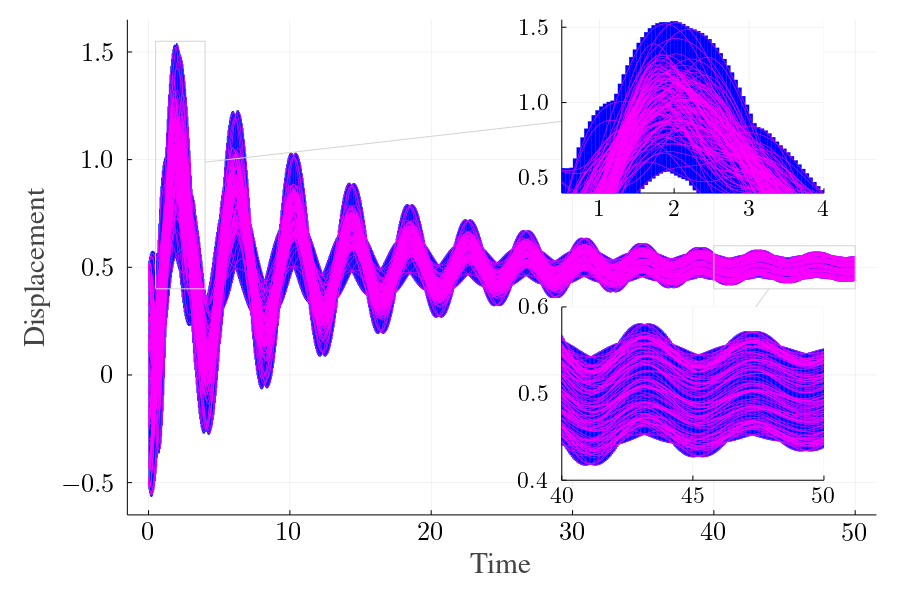
\includegraphics[width=0.82\linewidth,keepaspectratio]{example/displacement_vs_time}
	
	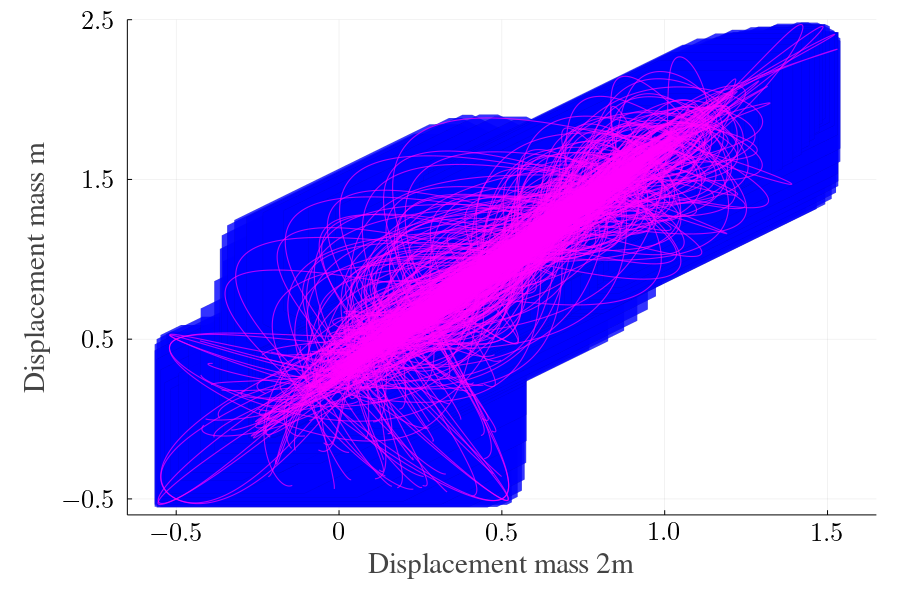
\includegraphics[width=0.82\linewidth,keepaspectratio]{example/displacement_vs_displacement}
	%
	\caption{Solution sets of mass $2m$ vs time (top) and displacement of both masses (bottom).}
	\label{fig:example}
\end{figure}



\begin{lstlisting}[label=ejemplo, numbers=left, aboveskip=0.55cm, belowskip=0.5cm]
	using ReachabilityAnalysis
	m = 0.25; k = 2.0
	M = [2m 0; 0 m]; K = [2k -k; -k k]; C = (M+K)/20
	F = [0.0, 1.0]; ΔF0 = Interval(0.9, 1.1)
	U0 = BallInf(zeros(4), 0.5)
	sys = SecondOrderLinearContinuousSystem(M, C, K, F)
	prob = InitialValueProblem(homogenize(sys), U0 × ΔF0)
	solA = solve(prob, 50, LGG09(δ=5e-2, dirs=:box, dim=5))
	solB = solve(prob, 50, LGG09(δ=5e-2, dirs=:oct, dim=5))
\end{lstlisting}

\noindent \emph{Perspectives.} We envision modeling uncertainties in density or stiffness using interval methods~\cite{forets2021intervalmat, ferranti2021interval}, as well as integrating our work with Julia's FEM projects~\cite{Gridap,Ferrite,FinEtools}.

% **************GENERATED FILE, DO NOT EDIT**************

\bibliographystyle{juliacon}
\bibliography{ref.bib}

	
\end{document}
